% !TEX root = main.tex
\subsection{1D MRI}
\label{sec:1DMRIkapitel}
Bei dem MRI-Verfahren wird neben dem Erdmagnetfeld $B_0$ ein Gradientenfeld \textbf{G} angelegt.
Somit ist die Larmorfrequenz nicht nur durch $B_0$ gegeben.
Es muss zusätzlich noch das angelegte Gradientenfeld mitbetrachtet werden.
Falls man dies speziell in x-Richtung (also $G_xx$) betrachtet, so kann die Larmorfrequenz wie folgt ausgedrückt werden:
\begin{align}
    \omega(x)=\gamma |B(x)|= \gamma \left(B_0+G_xx\right) \label{eq:gradientlarmor}
\end{align}
Aus dieser Formel geht nun hervor, dass jeder Spin ein vom Ort abhängiges Magnetfeld erfährt.
Somit besitzt jeder Spin eine andere Larmorfrequenz.
Diese präzidieren mit unterschiedlicher Geschwidigkeiten womit dann auf den Ort des Spins zurück geschlossen werden kann. \\

Die Grundidee wie dies am Ende gemesen wird liegt darin, dass man im Fourieraum ein Spektrum erhälten, indem Datenpunkte in Abhängigkeit von der Zeit gemessen werden und diese dann integriert werden.
Für die positiven Zeiten stellt dies kein Problem dar.
Jedoch wird bei der Fourietransformation auch über die negative Zeiten integriert, die nicht gemessen werden können.
Die Lösung dieses Problemes liegt darin, dass als erstes ein negatives Gradientenfeld $-G$ angelegt wird.
Was dies anschaulich bedeutet, kann in der folgenden Abbildung \ref{fig:1DMRI} sichtbar gemacht werden.  
\begin{figure}[H]
    \centering
    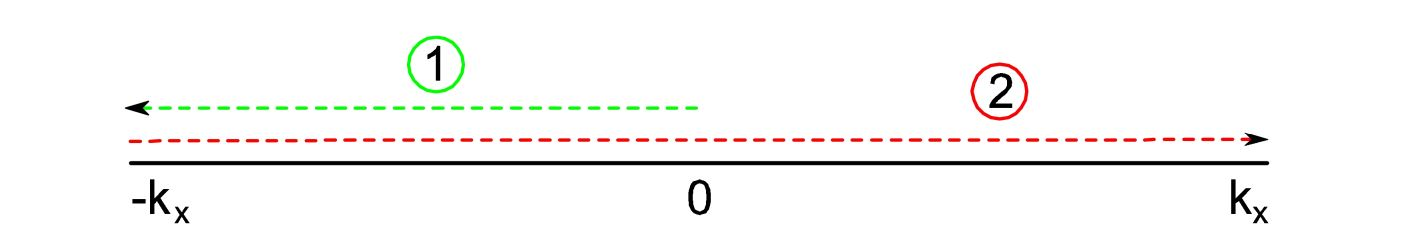
\includegraphics[width=0.8\textwidth]{Abbildungen/1DMRIkraum.JPG}
    \caption[Veranschaulichter Verlauf des k-Vektors im 1D-MRI]{Diese Abbildung dient zur Veranschaulichung der Messmethode im k-Raum.
    In Schritt 1 wird als erstes ein negativer Gradient angelegt, sodass im k-Raum der k-Vektor verringert wird.
    Das negative Gradientenfeld wird nun so lange angelegt, bis man die erwünschte Bandbreite in $-k_{x}$-Richtung erreicht hat.
    Sobald dies geschehen ist, wird das gleiche Gradientenfeld nur in positiver Richtung nochmal angelegt.
    Dies passiert so lange,  bis man im k-Raum die erwünschte Bandbreite von $-k_{x}$ bis $k_{x}$ erreicht hat.
    Das Signal wird hierbei während dem Vorgang (2) gemessen.\cite{Schmidt}}
    \label{fig:1DMRI}
\end{figure}

Als erstes wurde ein 1D-MRI in Richtung von der x-Achse gemessen.
Im folgenden werden nun zwei Messungen miteinander verglichen, die mit unterschiedlichen Parametern vermessen wurden.  
\begin{figure}[H]
    \centering
    % GNUPLOT: LaTeX picture with Postscript
\begingroup
  % Encoding inside the plot.  In the header of your document, this encoding
  % should to defined, e.g., by using
  % \usepackage[cp1252,<other encodings>]{inputenc}
  \inputencoding{cp1252}%
  \makeatletter
  \providecommand\color[2][]{%
    \GenericError{(gnuplot) \space\space\space\@spaces}{%
      Package color not loaded in conjunction with
      terminal option `colourtext'%
    }{See the gnuplot documentation for explanation.%
    }{Either use 'blacktext' in gnuplot or load the package
      color.sty in LaTeX.}%
    \renewcommand\color[2][]{}%
  }%
  \providecommand\includegraphics[2][]{%
    \GenericError{(gnuplot) \space\space\space\@spaces}{%
      Package graphicx or graphics not loaded%
    }{See the gnuplot documentation for explanation.%
    }{The gnuplot epslatex terminal needs graphicx.sty or graphics.sty.}%
    \renewcommand\includegraphics[2][]{}%
  }%
  \providecommand\rotatebox[2]{#2}%
  \@ifundefined{ifGPcolor}{%
    \newif\ifGPcolor
    \GPcolorfalse
  }{}%
  \@ifundefined{ifGPblacktext}{%
    \newif\ifGPblacktext
    \GPblacktexttrue
  }{}%
  % define a \g@addto@macro without @ in the name:
  \let\gplgaddtomacro\g@addto@macro
  % define empty templates for all commands taking text:
  \gdef\gplbacktext{}%
  \gdef\gplfronttext{}%
  \makeatother
  \ifGPblacktext
    % no textcolor at all
    \def\colorrgb#1{}%
    \def\colorgray#1{}%
  \else
    % gray or color?
    \ifGPcolor
      \def\colorrgb#1{\color[rgb]{#1}}%
      \def\colorgray#1{\color[gray]{#1}}%
      \expandafter\def\csname LTw\endcsname{\color{white}}%
      \expandafter\def\csname LTb\endcsname{\color{black}}%
      \expandafter\def\csname LTa\endcsname{\color{black}}%
      \expandafter\def\csname LT0\endcsname{\color[rgb]{1,0,0}}%
      \expandafter\def\csname LT1\endcsname{\color[rgb]{0,1,0}}%
      \expandafter\def\csname LT2\endcsname{\color[rgb]{0,0,1}}%
      \expandafter\def\csname LT3\endcsname{\color[rgb]{1,0,1}}%
      \expandafter\def\csname LT4\endcsname{\color[rgb]{0,1,1}}%
      \expandafter\def\csname LT5\endcsname{\color[rgb]{1,1,0}}%
      \expandafter\def\csname LT6\endcsname{\color[rgb]{0,0,0}}%
      \expandafter\def\csname LT7\endcsname{\color[rgb]{1,0.3,0}}%
      \expandafter\def\csname LT8\endcsname{\color[rgb]{0.5,0.5,0.5}}%
    \else
      % gray
      \def\colorrgb#1{\color{black}}%
      \def\colorgray#1{\color[gray]{#1}}%
      \expandafter\def\csname LTw\endcsname{\color{white}}%
      \expandafter\def\csname LTb\endcsname{\color{black}}%
      \expandafter\def\csname LTa\endcsname{\color{black}}%
      \expandafter\def\csname LT0\endcsname{\color{black}}%
      \expandafter\def\csname LT1\endcsname{\color{black}}%
      \expandafter\def\csname LT2\endcsname{\color{black}}%
      \expandafter\def\csname LT3\endcsname{\color{black}}%
      \expandafter\def\csname LT4\endcsname{\color{black}}%
      \expandafter\def\csname LT5\endcsname{\color{black}}%
      \expandafter\def\csname LT6\endcsname{\color{black}}%
      \expandafter\def\csname LT7\endcsname{\color{black}}%
      \expandafter\def\csname LT8\endcsname{\color{black}}%
    \fi
  \fi
    \setlength{\unitlength}{0.0500bp}%
    \ifx\gptboxheight\undefined%
      \newlength{\gptboxheight}%
      \newlength{\gptboxwidth}%
      \newsavebox{\gptboxtext}%
    \fi%
    \setlength{\fboxrule}{0.5pt}%
    \setlength{\fboxsep}{1pt}%
\begin{picture}(7200.00,5040.00)%
    \gplgaddtomacro\gplbacktext{%
      \csname LTb\endcsname%%
      \put(1078,704){\makebox(0,0)[r]{\strut{}$0$}}%
      \put(1078,1292){\makebox(0,0)[r]{\strut{}$5000$}}%
      \put(1078,1880){\makebox(0,0)[r]{\strut{}$10000$}}%
      \put(1078,2468){\makebox(0,0)[r]{\strut{}$15000$}}%
      \put(1078,3055){\makebox(0,0)[r]{\strut{}$20000$}}%
      \put(1078,3643){\makebox(0,0)[r]{\strut{}$25000$}}%
      \put(1078,4231){\makebox(0,0)[r]{\strut{}$30000$}}%
      \put(1078,4819){\makebox(0,0)[r]{\strut{}$35000$}}%
      \put(1385,484){\makebox(0,0){\strut{}$-30$}}%
      \put(2259,484){\makebox(0,0){\strut{}$-20$}}%
      \put(3133,484){\makebox(0,0){\strut{}$-10$}}%
      \put(4007,484){\makebox(0,0){\strut{}$0$}}%
      \put(4880,484){\makebox(0,0){\strut{}$10$}}%
      \put(5754,484){\makebox(0,0){\strut{}$20$}}%
      \put(6628,484){\makebox(0,0){\strut{}$30$}}%
    }%
    \gplgaddtomacro\gplfronttext{%
      \csname LTb\endcsname%%
      \put(198,2761){\rotatebox{-270}{\makebox(0,0){\strut{}Amplitude in $\si{\milli \second}$}}}%
      \put(4006,154){\makebox(0,0){\strut{}Frequenz in $\si{\hertz}$}}%
      \csname LTb\endcsname%%
      \put(5816,4646){\makebox(0,0)[r]{\strut{}1D-MRI Messung, angepasste FOV und Bandbreite  }}%
    }%
    \gplbacktext
    \put(0,0){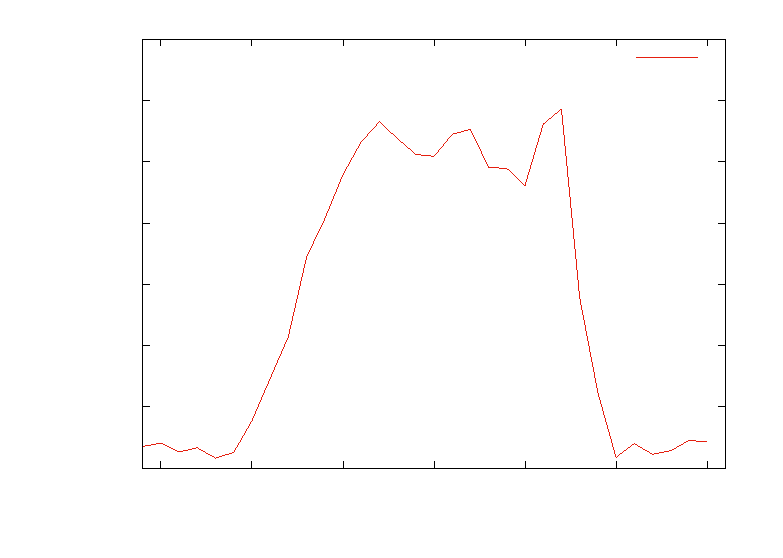
\includegraphics{plots/1DMRI}}%
    \gplfronttext
  \end{picture}%
\endgroup

    \caption[1D-MRI in x-Richtung nach Anpassung der FOV und Bandbreite]{1D-MRI in x-Richtung nach Anpassung der FOV und Bandbreite. Aus dieser Abbildung wurde eine Länge des Phantoms von $l=\SI{15,65}{\centi\m}$ ermittelt. Ein Peak ist bei ca. $\SI{13}{\hertz}$ zu sehen, welches auf ein Vielfaches der deutschen Netzspannung ($\SI{50}{\hertz}$) ergibt, da es sich hierbei um $\SI{1850}{\hertz}$. Es ist ein steiler Anstieg/Abfall um $\pm \SI{20}{\hertz}$ zu sehen, was auf eine \glqq rechteckige\grqq Form des Objektes entlang der x-Achse schließen lässt.\label{fig:1Dx}}
\end{figure}
% In der Abbildung \ref{fig:1Dx} kann man große unterschiede zwischen den beiden Messungen sehen. Es ist hierbei schwer aus der ersten Messung gute Informationen über das Phantom heraus zu bekommen. Es ist kein klarer Abfall zu sehen, weshalb man daraus nicht die Abmessung des Phantomes herausbekommen kann.
In der Abbildung \ref{fig:1Dx} ist zu sehen, dass bei $\SI{-20}{\hertz}$ und $\SI{20}{\hertz}$ ein starker Anstieg/Abfall des Signals stattfindet. Dies lässt sich dadurch erklären, dass durch die räumliche Ausdehnung des Phantoms die Spins an unterschiedlichen Orten eine andere Larmorfrequenz besitzten. Ursache hierfür ist das Gradientenfeld, welches während dem Messvorgang angelegt ist. Diese unterschiedlichen Larmorfrequenzen stellen das \glqq Plateau\grqq \, dar, was zwischen $\SI{-20}{\hertz}$ und $\SI{20}{\hertz}$ vorhanden ist.\\
Anhand dieses Signales kann  nun auch die Größe des Objektes ermittelt werden. Hierzu wird die Formel \ref{eq:gradientlarmor} benutzt um $\Delta x$ zu berechnen. Hierbei wird $\Delta\omega= 2\pi \Delta f$ umgerechnet, sodass man die folgende Formel erhält:
\begin{align}
    \Delta x&=\frac{\Delta\omega}{\gamma G_x}\\
    \Delta x&=\frac{\Delta f \cdot 2\pi}{\gamma G_x}\\
\end{align}\label{eq:FOV}
Aus der Abbildung kann die Bandbreite von ca. $\SI{40}{\hertz}$ ermittelt werden. Das gyromagnetische Moment von $\SI{2.67e8}{\s^{-1}\tesla^{-1}}$ wurde aus \cite{Schmidt} entnommen und der Gradient $G_x=\SI{6,0}{\frac{\mu\tesla}{\m}}$ wurde am Versuchstag im Messprotokoll festgehalten. Mit diesen Daten bekommt man für die Länge des Phantomes $l=\SI{15,65}{\centi\m}$ heraus.\\
Neben der Bandbreite kann in der Abbildung beobeachtet werden, dass bei ca. $\SI{13}{\hertz}$ ein kleiner Peak zu sehen ist.(Dieser Peak ist wesentlich deutlicher noch in Abb. \ref{fig:1Dy} zu sehen). Der Ursprung dieser Peaks liegt an der deutschen Netzspannung, die mit $\SI{50}{\hertz}$ getaktet ist. Wenn man sich nun den Urprung anschaut, so liegt dieser bei der Larmorfrequenz von $\SI{1837,27}{\hertz}$, die am ersten Versuchstag vermessen wurde. Wenn dazu noch $\SI{13}{\hertz}$ hinzu addiert werden, so  kommt man zu dem Schluss, dass die Peaks bei $\SI{1850}{\hertz}$ liegen und somit ein Vielfaches von der Netzspannung sind.\\
Wie schon im vorherigen Absatz angesprochen, wurde im Anschluss eine weitere MRI Messung gemacht, die sich jedoch entlang der y-Achse orientiert hat. Die Messung wird nun in der folgenden Abbildung dargestellt.
\begin{figure}[H]
    \centering
    % GNUPLOT: LaTeX picture with Postscript
\begingroup
  % Encoding inside the plot.  In the header of your document, this encoding
  % should to defined, e.g., by using
  % \usepackage[cp1252,<other encodings>]{inputenc}
  \inputencoding{cp1252}%
  \makeatletter
  \providecommand\color[2][]{%
    \GenericError{(gnuplot) \space\space\space\@spaces}{%
      Package color not loaded in conjunction with
      terminal option `colourtext'%
    }{See the gnuplot documentation for explanation.%
    }{Either use 'blacktext' in gnuplot or load the package
      color.sty in LaTeX.}%
    \renewcommand\color[2][]{}%
  }%
  \providecommand\includegraphics[2][]{%
    \GenericError{(gnuplot) \space\space\space\@spaces}{%
      Package graphicx or graphics not loaded%
    }{See the gnuplot documentation for explanation.%
    }{The gnuplot epslatex terminal needs graphicx.sty or graphics.sty.}%
    \renewcommand\includegraphics[2][]{}%
  }%
  \providecommand\rotatebox[2]{#2}%
  \@ifundefined{ifGPcolor}{%
    \newif\ifGPcolor
    \GPcolorfalse
  }{}%
  \@ifundefined{ifGPblacktext}{%
    \newif\ifGPblacktext
    \GPblacktexttrue
  }{}%
  % define a \g@addto@macro without @ in the name:
  \let\gplgaddtomacro\g@addto@macro
  % define empty templates for all commands taking text:
  \gdef\gplbacktext{}%
  \gdef\gplfronttext{}%
  \makeatother
  \ifGPblacktext
    % no textcolor at all
    \def\colorrgb#1{}%
    \def\colorgray#1{}%
  \else
    % gray or color?
    \ifGPcolor
      \def\colorrgb#1{\color[rgb]{#1}}%
      \def\colorgray#1{\color[gray]{#1}}%
      \expandafter\def\csname LTw\endcsname{\color{white}}%
      \expandafter\def\csname LTb\endcsname{\color{black}}%
      \expandafter\def\csname LTa\endcsname{\color{black}}%
      \expandafter\def\csname LT0\endcsname{\color[rgb]{1,0,0}}%
      \expandafter\def\csname LT1\endcsname{\color[rgb]{0,1,0}}%
      \expandafter\def\csname LT2\endcsname{\color[rgb]{0,0,1}}%
      \expandafter\def\csname LT3\endcsname{\color[rgb]{1,0,1}}%
      \expandafter\def\csname LT4\endcsname{\color[rgb]{0,1,1}}%
      \expandafter\def\csname LT5\endcsname{\color[rgb]{1,1,0}}%
      \expandafter\def\csname LT6\endcsname{\color[rgb]{0,0,0}}%
      \expandafter\def\csname LT7\endcsname{\color[rgb]{1,0.3,0}}%
      \expandafter\def\csname LT8\endcsname{\color[rgb]{0.5,0.5,0.5}}%
    \else
      % gray
      \def\colorrgb#1{\color{black}}%
      \def\colorgray#1{\color[gray]{#1}}%
      \expandafter\def\csname LTw\endcsname{\color{white}}%
      \expandafter\def\csname LTb\endcsname{\color{black}}%
      \expandafter\def\csname LTa\endcsname{\color{black}}%
      \expandafter\def\csname LT0\endcsname{\color{black}}%
      \expandafter\def\csname LT1\endcsname{\color{black}}%
      \expandafter\def\csname LT2\endcsname{\color{black}}%
      \expandafter\def\csname LT3\endcsname{\color{black}}%
      \expandafter\def\csname LT4\endcsname{\color{black}}%
      \expandafter\def\csname LT5\endcsname{\color{black}}%
      \expandafter\def\csname LT6\endcsname{\color{black}}%
      \expandafter\def\csname LT7\endcsname{\color{black}}%
      \expandafter\def\csname LT8\endcsname{\color{black}}%
    \fi
  \fi
    \setlength{\unitlength}{0.0500bp}%
    \ifx\gptboxheight\undefined%
      \newlength{\gptboxheight}%
      \newlength{\gptboxwidth}%
      \newsavebox{\gptboxtext}%
    \fi%
    \setlength{\fboxrule}{0.5pt}%
    \setlength{\fboxsep}{1pt}%
\begin{picture}(7200.00,5040.00)%
    \gplgaddtomacro\gplbacktext{%
      \csname LTb\endcsname%%
      \put(1078,704){\makebox(0,0)[r]{\strut{}$0$}}%
      \put(1078,1260){\makebox(0,0)[r]{\strut{}$5000$}}%
      \put(1078,1816){\makebox(0,0)[r]{\strut{}$10000$}}%
      \put(1078,2372){\makebox(0,0)[r]{\strut{}$15000$}}%
      \put(1078,2928){\makebox(0,0)[r]{\strut{}$20000$}}%
      \put(1078,3484){\makebox(0,0)[r]{\strut{}$25000$}}%
      \put(1078,4040){\makebox(0,0)[r]{\strut{}$30000$}}%
      \put(1078,4597){\makebox(0,0)[r]{\strut{}$35000$}}%
      \put(1539,484){\makebox(0,0){\strut{}$-15$}}%
      \put(2362,484){\makebox(0,0){\strut{}$-10$}}%
      \put(3184,484){\makebox(0,0){\strut{}$-5$}}%
      \put(4007,484){\makebox(0,0){\strut{}$0$}}%
      \put(4829,484){\makebox(0,0){\strut{}$5$}}%
      \put(5652,484){\makebox(0,0){\strut{}$10$}}%
      \put(6474,484){\makebox(0,0){\strut{}$15$}}%
    }%
    \gplgaddtomacro\gplfronttext{%
      \csname LTb\endcsname%%
      \put(198,2761){\rotatebox{-270}{\makebox(0,0){\strut{}Amplitude in $\si{\milli \second}$}}}%
      \put(4006,154){\makebox(0,0){\strut{}Frequenz in $\si{\hertz}$}}%
      \csname LTb\endcsname%%
      \put(5816,4646){\makebox(0,0)[r]{\strut{}erste 1D MRI Messung in yRichtung}}%
      \csname LTb\endcsname%%
      \put(5816,4426){\makebox(0,0)[r]{\strut{}zweite 1D MRI Messung mit ver\"anderter5 Bandbreite}}%
    }%
    \gplbacktext
    \put(0,0){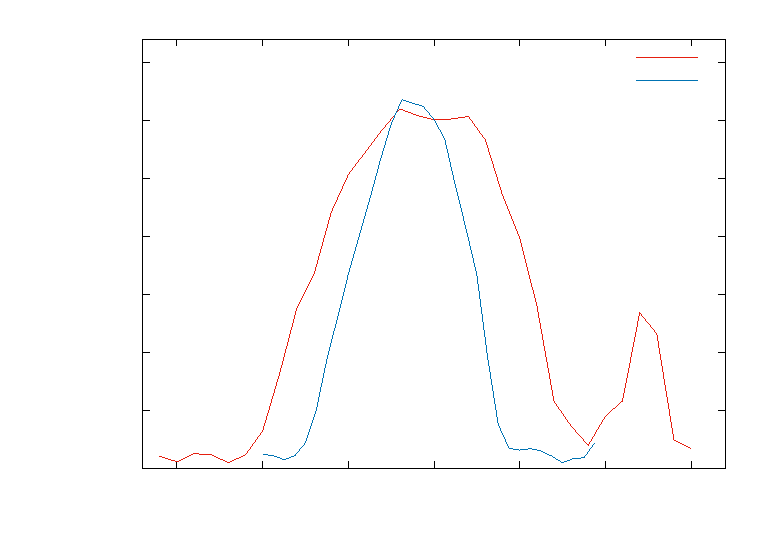
\includegraphics{plots/1DMRIy}}%
    \gplfronttext
  \end{picture}%
\endgroup

    \caption[1-MRI in y-Richtung nach Anpassung der FOV]{1-MRI in y-Richtung nach Anpassung der FOV. Hier wurde eine Breite von $b=\SI{6,57}{\centi \m}$ bwatimmt. Der Anstieg/Abfall ist nicht steil, was eher auf eine runde Form des Phantoms spricht entlang der y-Achse}\label{fig:1Dy}
\end{figure} 
Auch hier kann beobachtet werden, dass die räumliche Ausdehnung der Probe zu einer Erhöhung des Signals führt. Die Breite des Phantoms $b=\SI{6,57}{\centi \m}$ wurde analog zu der Formel \ref{eq:FOV} wie vorhin berechnet. Wenn die Signale in x,y-Richtung verglichen werden, so sieht man tendenziell, dass das Signal entlang der x-Richtung schneller bzw. stärker ansteigt/abfällt. Dies könnte unter anderem mit der Form des Phantoms zusammen hängen. Hierbei würde ein starker Abfall eher auf eine eckige Form zutreffen und eine schwächerer Abfall würde eher auf eine runde Form zutreffen. Mit diesem Wissen kann man die Vermutung aufstellen, dass das Phantom ein Zylinder sein kann. Dies würde erklären, dass entlang der x-Richtung der Graph stärker abflällt, da ein Zylinder entlang der Höhe einem Rechteck ähnlicher sieht als einer Kugel oder einem Kreis. Wenn jedoch die Grundfläche in der y,z-Ebene betrachtet wird, so handelt es sich hierbei um einen Kreis. Dies würde erklären, warum das Signal in y-Richtung schwächer ansteigt/abfällt. Wenn man mit diesem Wissen das Volumen des Zylinders mit der ermittelten Länge und der Breite berechnet, so erhält man ein Volumen $V=\SI{532}{\milli\liter}$.\\
In anderen Versuchsteilen wurde ein ähnliches Objekt verwendet, welches ein Volumen von $\SI{500}{\milli \liter}$ hatte. Die Vermutung liegt nahe, dass das untersuchte Phantom die gleiche Abmessung hatte und ebenfalls mit Wasser gefüllt war. Die Abweichung von $\SI{32}{\milli\liter}$ können durch Messunsicherheiten erklärt werden.\\
Eine mögliche Quelle für eine Unsicherheit kann durch das Auflösungsvermögen entstehen. Das Auflösungsvermögen ist durch $\Delta x=\frac{FOV}{N}$ gegeben, wobei N die Anzahl der Pixels darstellt\cite{Schmidt}. Nun könnte man diesen Wert bestimmen, aber dies würde aus zwei Gründen nicht so viel Sinn machen. Zum einen wäre es der Fakt, dass zwar ein Wert ermittelt werden kann, aber da es keine Referenzwerte gibt, womit man entscheiden könnte, ob dies eine gute Auflösung ist oder nicht, wurde dies nicht gemacht. Der andere Grund, warum dies nicht explizit berechnet wurde liegt daran, dass es meist auch andere Faktoren gibt, die bei der tatsächlichen Auflösung eine Rolle spielen. Hierbei kann es sein, dass zwischen den einzelnen Pixels es zu einer unschärfe kommt, wodurch die Auflösung dann gröber wird.\\
Ein weiteres Problem stellt sich bei der Auswertung heraus. Hierbei ist es schwierig, genau zu identifizieren, wo genau das Phantom aufhört bzw. die Bandbreite zu bestimmen. Hier muss man darauf ahcten, dass das Signal von der Netztfrequenz oder auch von dem Rauschen nicht dazu genommen werden soll. Vor allem in der ersten Abbildung stellt dies ein Problem dar, da sich das Phantom mit dem Peak der Netzfrequenz überschneidet.
Wenn man die Unsicherheit kleiner haben möchte, dann kann man versuchen die Auflösung zu verbessern indem man die FOV (den Bereich den man anschaut) kleiner wählt und somit nur das Phantom vermisst. Darauf wurde am Versuchstag schon geachtet, dass dies möglichst gut eingehalten wird. \\
Eine weiter Möglichkeit das Signal zu verbessern besteht darin, indem man mehrere Messungen hintereinander macht. Dadurch hätte man mehr Datenpunkte zur Verfügung, womit man ein gemitteltes Signal bekommen würde. Dies macht bis zu einem gewissen Grad Sinn, jedoch muss darauf geachtet werden, dass die Messungen nicht \glqq ineffizient\grqq werden. Hierbei ist die Effizient abhängig von der Anzahl der Messungen und der damit verbundenen Messzeit. Mit der Häufigkeit der Messungen wird versucht, das Signal-Rausch-Verhältnis so klein wie möglich zu machen. Für eine Anzahl von N Messungen wird diese um $\sqrt{N}$ verbessert, wobei die Anzahl der Messungen sich in der gemessenen Zeit dann wiederspiegelt. Mit dieser Überlegung erhält man, dass die Effizienz$\propto\frac{SNR}{\sqrt{\text{Messzeit}}}$ ist. Es macht somit nicht immer Sinn, die Anzahl der Messungen zu erhöhen, da sonst das Signal zu Rausch Verhältnis zu klein wird und somit nicht mehr effizient ist.
Wenn ein 2D-MRI gemacht wird, ist die Effizienz noch wichtiger, da sonst die Messungen zu lange dauern würde und die gemessenen Daten dies nicht rechtfertigen würden. 